% !TeX spellcheck = en_US
% !TeX encoding = utf8
% !TeX program = xelatex
% !BIB program = bibtex

\documentclass[notes]{beamer}
% \documentclass[draft]{beamer}	
\usetheme{Singapore}
% \usetheme{Hannover}
%\usepackage{pgfpages}
%\setbeameroption{show notes on second screen}

\usepackage[british]{babel}
\usepackage{graphicx,hyperref,url}
% \usepackage{ru}
\usepackage{mmstyles}
% \usepackage{hanging}
\usepackage{listings}
\usefonttheme[onlymath]{serif}
\usepackage{fontspec}
\usepackage{xeCJK}
% \pgfdeclareimage[width=\paperwidth,height=\paperheight]{bg}{background}
% \setbeamertemplate{background}{\pgfuseimage{bg}}
%% columns
\newcommand{\begincols}[1]{\begin{columns}{#1}}
\newcommand{\stopcols}{\end{columns}}
% \usepackage[backend=biber]{biblatex}
% \bibliography{./ref.bib}
%\addbibresource{ref.bib}
\usepackage{indentfirst}
\usepackage{longtable}
\usepackage{float}
%\usepackage{picins}
\usepackage{rotating}
\usepackage{subfigure}
\usepackage{tabu}
\usepackage{amsmath}
\usepackage{amssymb}
\usepackage{setspace}
\usepackage{amsfonts}
\usepackage{appendix}
\usepackage{listings}
\usepackage{xcolor}
\usepackage{geometry}
% \setCJKfamilyfont{cjkhwxk}{SimSun}
% \newcommand*{\cjkhwxk}{\CJKfamily{cjkhwxk}}
%\newfontfamily{\consolas}{Consolas}
%\newfontfamily{\monaco}{Monaco}
%\setmonofont[Mapping={}]{Consolas}	%英文引号之类的正常显示,相当于设置英文字体
%\setsansfont{Consolas} %设置英文字体 Monaco, Consolas,  Fantasque Sans Mono
% \setmainfont{Times New Roman}
% \newfontfamily{\consolas}{Times New Roman}
% \newfontfamily{\monaco}{Arial}
% \setCJKmainfont{Times New Roman}
%\setmainfont{MONACO.TTF}
%\setsansfont{MONACO.TTF}
\newcommand{\verylarge}{\fontsize{60pt}{\baselineskip}\selectfont}  
\newcommand{\chuhao}{\fontsize{44.9pt}{\baselineskip}\selectfont}  
\newcommand{\xiaochu}{\fontsize{38.5pt}{\baselineskip}\selectfont}  
\newcommand{\yihao}{\fontsize{27.8pt}{\baselineskip}\selectfont}  
\newcommand{\xiaoyi}{\fontsize{25.7pt}{\baselineskip}\selectfont}  
\newcommand{\erhao}{\fontsize{23.5pt}{\baselineskip}\selectfont}  
\newcommand{\xiaoerhao}{\fontsize{19.3pt}{\baselineskip}\selectfont} 
\newcommand{\sihao}{\fontsize{14pt}{\baselineskip}\selectfont}      % 字号设置  
\newcommand{\xiaosihao}{\fontsize{12pt}{\baselineskip}\selectfont}  % 字号设置  
\newcommand{\wuhao}{\fontsize{10.5pt}{\baselineskip}\selectfont}    % 字号设置  
\newcommand{\xiaowuhao}{\fontsize{9pt}{\baselineskip}\selectfont}   % 字号设置  
\newcommand{\liuhao}{\fontsize{7.875pt}{\baselineskip}\selectfont}  % 字号设置  
\newcommand{\qihao}{\fontsize{5.25pt}{\baselineskip}\selectfont}    % 字号设置 

\graphicspath{{./fig/}}

% \setbeamertemplate{footnote}{%
%   \hangpara{2em}{1}%
%   \makebox[2em][l]{\insertfootnotemark}\footnotesize\insertfootnotetext\par%
% }

\definecolor{cred}{rgb}{0.6,0,0}
\definecolor{cgreen}{rgb}{0.25,0.5,0.35}
\definecolor{cpurple}{rgb}{0.5,0,0.35}
\definecolor{cdocblue}{rgb}{0.25,0.35,0.75}
\definecolor{cdark}{rgb}{0.95,1.0,1.0}
\lstset{
	language=R,
	numbers=left,
	numberstyle=\tiny\color{black},
	keywordstyle=\color{cpurple}\consolas,
	commentstyle=\color{cgreen}\consolas,
	stringstyle=\color{cred}\consolas,
	frame=single,
	escapeinside=``,
	xleftmargin=1em,
	xrightmargin=1em, 
	backgroundcolor=\color{cdark},
	aboveskip=1em,
	breaklines=true,
	tabsize=3
} 

\providecommand{\tightlist}{%
  \setlength{\itemsep}{0pt}\setlength{\parskip}{0pt}}

  
% The title of the presentation:
%  - first a short version which is visible at the bottom of each slide;
%  - second the full title shown on the title slide;
\title[Opt for ML]{Regression \& the LMS Algorithm}

% Optional: a subtitle to be dispalyed on the title slide
% \subtitle{Optimization for Machine Learning}

% The author(s) of the presentation:
%  - again first a short version to be displayed at the bottom;
%  - next the full list of authors, which may include contact information;
\author[YingmingLi]{Yingming Li \\ yingming@zju.edu.cn}
% The institute:
%  - to start the name of the university as displayed on the top of each slide
%    this can be adjusted such that you can also create a Dutch version
%  - next the institute information as displayed on the title slide

\institute[DSERC, ZJU]{Data Science \& Engineering Research Center, ZJU}

% Add a date and possibly the name of the event to the slides
%  - again first a short version to be shown at the bottom of each slide
%  - second the full date and event name for the title slide
\date[\today]{\today}

\begin{document}

\AtBeginSection[]
{
	\begin{frame}
		\frametitle{Outline}
		\tableofcontents[currentsection]
	\end{frame}
}

% \AtBeginSubsection[2-]
% {
%    \begin{frame}
%        \frametitle{Outline}
%        \tableofcontents[currentsection]
%    \end{frame}
% }


\begin{frame}
	\titlepage
	\begin{center}
		Adapted from slides provided by Prof.  Michael Mandel.		
	\end{center}

\end{frame}

\section{}\label{section}

\begin{frame}{Problem statement}

\centering 

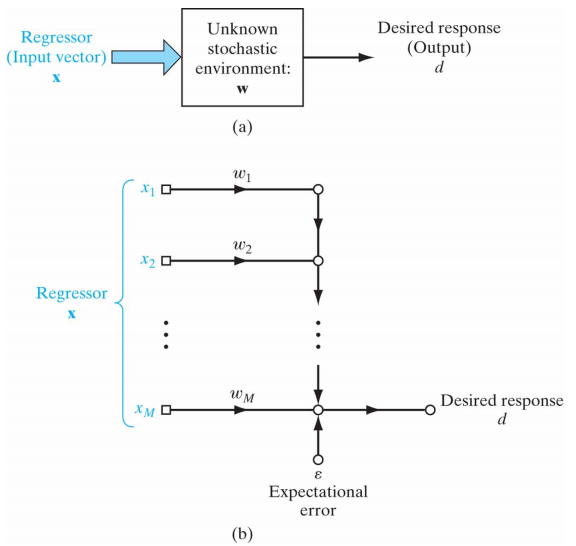
\includegraphics[width=0.65000\textwidth]{2018-03-09-15-26-11.png} ~

\end{frame}

\begin{frame}{Linear regression with one variable}

Given a set of \(N\) pairs of data \(\{x_i,d_i\}\), approximate \(d\) by
a linear function of \(x\) (regressor), \ie, \[d \approx wx +b\] or

\begin{equation*}
\begin{aligned}
d_i &= y_i + \epsilon_i  = \varphi (wx_i + b ) + \varepsilon \\ 
 & = wx_i + b+\varepsilon 
\end{aligned}
\end{equation*}

where the activation function \(\varphi(x) = x\) is a linear function,
corresponding to a linear neuron. \(y\) is the output of the neuron, and
\[\varepsilon_i = d_i -y_i\] is called the (expectational) regression
error.

\end{frame}

\begin{frame}{Linear regression}

\begin{itemize}
\tightlist
\item
  The problem of regression with one variable is how to choose \(w\) and
  \(b\) to minimize the regression error.
\item
  The least squares method aims to minimize the square error
\end{itemize}

\[E=\frac{1}{2}\sum_{i=1}^{N} \varepsilon_i^2 = \frac{1}{2} \sum_{i=1}^{N} (d_i -y_i)^2\]

\end{frame}

\begin{frame}{Linear regression}

To minimize the two-variable square function, set

\[\left\{\begin{array}{cc}
\frac{\partial E}{\partial b} & =0 \\ 
\frac{\partial E}{\partial w} & =0 
\end{array} \right.\]

\[\Rightarrow \left\{\begin{array}{cc}
-\sum_{i}(d_i -wx_i -n) & =0 \\  
-\sum_{i} (d_i -wx_i -b) x_i & =0 
\end{array} \right.\]

\end{frame}

\begin{frame}{Analytic solution approaches}

\begin{itemize}
\tightlist
\item
  Solve one equation for \(b\) in terms of \(w\)

  \begin{itemize}
  \tightlist
  \item
    Substitute into other equation, solve for \(w\)
  \item
    Substitute solution for \(w\) back into equation for \(b\)
  \end{itemize}
\end{itemize}

\[\left\{\begin{array}{cc}
-\sum_{i}(d_i -wx_i -b) & =0 \\  
-\sum_{i} (d_i -wx_i -b) x_i & =0 
\end{array} \right.\]

\(\Rightarrow \quad\) \pause
\(b=\frac{\sum_i x_i^2 \sum_i d_i - \sum_i x_i \sum_i x_i d_i}{N \sum_i (x_i - \bar{x} )^2} , \quad\)
\(w=\frac{\sum_i (x_i - \bar{x}) (d_i - \bar{d}) }{\sum_i (x_i - \bar{x} )^2 }\)

, where an \(\bar{x}\) indicates the mean

There may exist other forms, such as \textcolor{red}{
$w=\frac{\sum_i d_i (x_i-\bar{x})}{\sum_i x_i^2 - \frac{1}{m} (\sum_i x_i)^2 }$, 
$w=\frac{\sum_i(d_i-\bar{d})x_i}{\sum_i (x_i-\bar{x})x_i}$ 
}

\end{frame}

\begin{frame}{Analytic solution approaches}

\begin{itemize}
\tightlist
\item
  Solve one equation for \(b\) in terms of \(w\)

  \begin{itemize}
  \tightlist
  \item
    Substitute into other equation, solve for \(w\)
  \item
    Substitute solution for \(w\) back into equation for \(b\)
  \end{itemize}
\item
  Setup system of equations in matrix notation

  \begin{itemize}
  \tightlist
  \item
    Solve matrix equation
  \end{itemize}
\item
  Rewrite problem in matrix form

  \begin{itemize}
  \tightlist
  \item
    Compute matrix gradient
  \item
    Solve for \(w\)
  \end{itemize}
\end{itemize}

\end{frame}

\begin{frame}{Linear regression in matrix notation}

Let \(\mX = [\vx_1 ,\vx_2 ,\vx_3 ,\dots ,\vx_N]^T\), then the model
predictions are \(\vy=\mX \vw\). And the mean square error can be
written as \[E(\vw)=\|\vd - \vy\|^2 = \|\vd -\mX \vw\|^2\]

To find the optimal \(\vw\), set the gradient of the error \wrt \(\vw\)
equal to 0 and solve for \(\vw\).

\[\partial E(\vw) / \partial \vw=0\]

\end{frame}

\begin{frame}{Linear regression in matrix notation}

\begin{equation*}
\begin{aligned}
\frac{\partial}{\partial \vw} E(\vw) & = \frac{\partial}{\partial \vw} \| \vd - \mX \vw \|^2 \\  
&= \frac{\partial}{\partial \vw} (\vd -\mX \vw)^T(\vd -\mX \vw) \\ 
&= \frac{\partial}{\partial \vw} \vd^T \vd \textcolor{red}{- \vd^T \mX \vw - \vw^T \mX^T \vd }+ \vw^T \mX^T \mX \vw \\ 
&=\textcolor{red}{ 2 \mX^T \mX \vw} -2 \mX^T \vd  = 0
\end{aligned}
\end{equation*}

\(\Rightarrow \vw = (\mX ^T \mX)^{-1} \mX^T \vd\)

\end{frame}

\begin{frame}{Finding optimal parameters via search}

\begin{itemize}
\tightlist
\item
  Often there is no closed form solution for
  \(\frac{\partial}{\partial \vw} E(\vw)=0\)
\item
  We can still use the gradient in a numerical solution
\item
  We will still use the same example to permit comparison
\item
  For simplicity's sake, set \(b = 0\)
\end{itemize}

\[E(w) = 1/2 \sum_{i=1}^{N} (d_i - wx_i)^2\]

, where \(E(w)\) is called cost function.

\end{frame}

\begin{frame}{Cost function}

\centering 

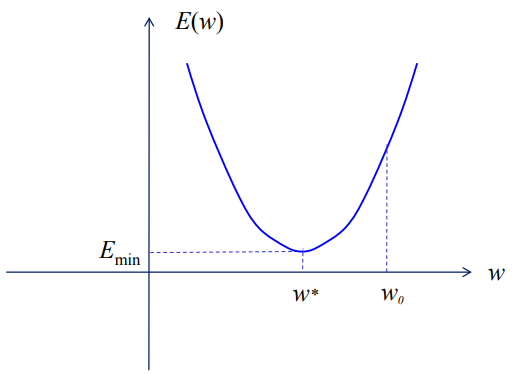
\includegraphics[width=0.50000\textwidth]{2018-03-09-22-15-39.png}\\

Question: how can we update \(w\) from \(w_0\) to minimize \(E\)?

\end{frame}

\begin{frame}{Gradient and directional derivatives}

Consider a two-variable function \(f(x,y)\). Its gradient at the point
\((x_0 ,y_0)^T\) is defined as

\begin{equation*}
    \begin{aligned}
        \nabla f & = \left. (\partial f(x,y) / \partial x , \partial f(x,y) / \partial y)^T \right|_{x=x_0,y=y_0}   \\ 
        & = f_x(x_0,y_0) \vu_x + f_y(x_0,y_0) \vu_y 
    \end{aligned}
\end{equation*}

, where \(\vu_x\) and \(\vu_y\) are unit vectors in the \(x\) and \(y\)
directions, and \(f_x=\partial f / \partial x\) and
\(f_y = \partial f / \partial y\)

\end{frame}

\begin{frame}{Gradient and directional derivatives}

At any given direction, \(\vu = \alpha \vu_x + b \vu_y\), with
\(\sqrt{a^2+b^2}=1\), the directional derivative at \((x_0, y_0 )^T\)
along the unit vector \(\vu\) is

\begin{equation*}
    \begin{aligned}
        D_\vu f(x_0,y_0) &= \lim_{h \rightarrow 0} \frac{f(x_0 + ha, y_0+hb)-f(x_0,y_0) }{h} \\  
        &= \lim_{h \rightarrow 0} \left[f(x_0+ha , y_0 +hb)-f(x_0,y_0+hb)\right]/h \\
         &\qquad \quad +\left[f(x_0,y_0+hb)-f(x_0,y_0)\right]/{h} \\
        &= af_x(x_0,y_0)+bf_y(x_0,y_0) \\
        &= \nabla f(x_0,y_0)^T \vu
    \end{aligned}
\end{equation*}

Which direction has the greatest slope? The gradient! Because of the dot
product.

\end{frame}

\begin{frame}{Gradient and directional derivatives}

Example: \(f(x,y)=5/2 x^2 -3xy + 5/2 y^2 +2x +2y\)

\centering 

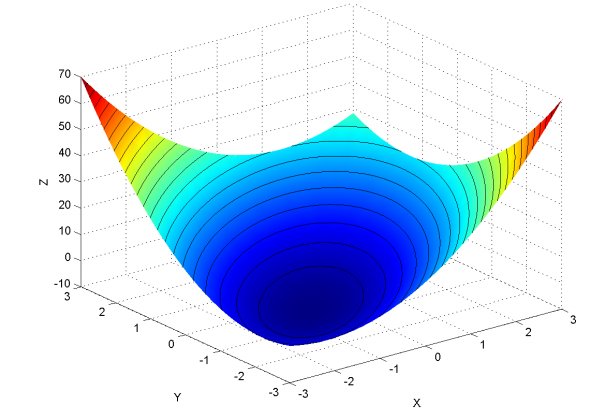
\includegraphics[width=0.70000\textwidth]{2018-03-09-22-31-32.png}\\

\end{frame}

\begin{frame}{Gradient and directional derivatives}

Example: \(f(x,y)=5/2 x^2 -3xy + 5/2 y^2 +2x +2y\)

\centering 

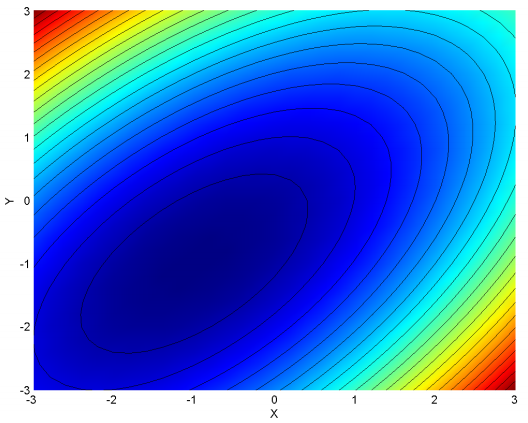
\includegraphics[width=0.70000\textwidth]{2018-03-09-22-34-05.png}\\

\end{frame}

\begin{frame}{Gradient and directional derivatives (cont.)}

\begin{itemize}
\tightlist
\item
  The level curves of a function \(f(x,y)\) are curves such that
  \(f(x,y)=k\)
\item
  Thus, the directional derivative along a level curve is 0
  \[D_\vu = \nabla f(x_0,y_0) ^T \vu = 0 \]
\item
  And the gradient vector is perpendicular to the level curve
\end{itemize}

\end{frame}

\begin{frame}{Gradient and directional derivatives (cont.)}

\begin{itemize}
\tightlist
\item
  The gradient of a cost function is a vector with the dimension of w
  that points to the direction of maximum \(E\) increase and with a
  magnitude equal to the slope of the tangent of the cost function along
  that direction

  \begin{itemize}
  \tightlist
  \item
    Can the slope be negative?
  \end{itemize}
\end{itemize}

\end{frame}

\begin{frame}{Gradient illustration}

\centering 

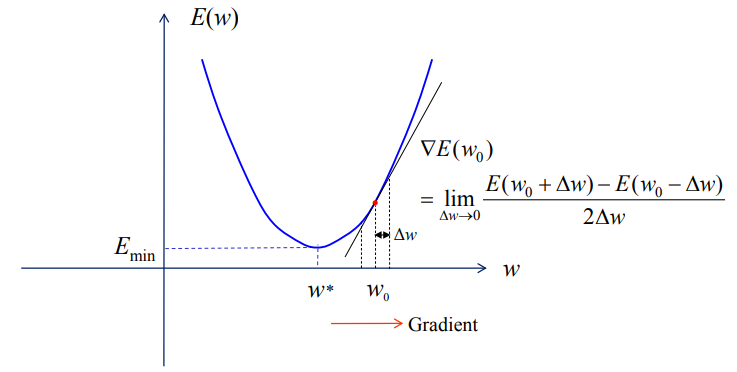
\includegraphics[width=0.80000\textwidth]{2018-03-10-09-23-28.png}\\

\end{frame}

\begin{frame}{Gradient descent}

\centering 

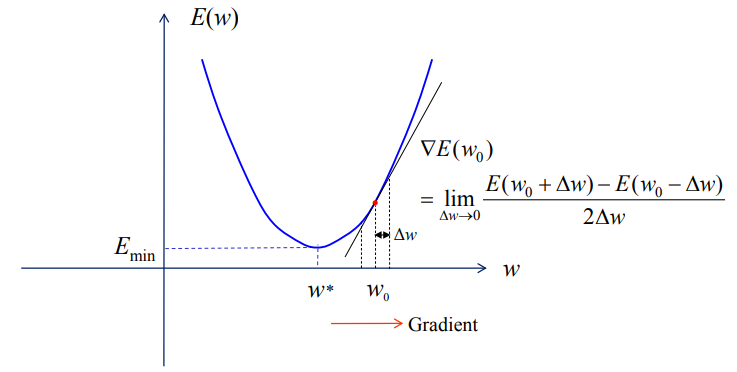
\includegraphics[width=0.80000\textwidth]{2018-03-10-09-23-28.png}\\

\begin{itemize}
\item
  Minimize the cost function via gradient (steepest) descent a case of
  hill-climbing \[w( n + 1) = w( n ) − \eta \nabla E ( n )\]

  \begin{itemize}
  \tightlist
  \item
    \(n\): iteration number
  \item
    \(\eta\): learning rate
  \end{itemize}
\end{itemize}

\end{frame}

\begin{frame}{Gradient descent (cont.)}

\begin{itemize}
\tightlist
\item
  For the mean-square-error cost function and linear neurons

  \begin{equation*}
  \begin{aligned}
      E ( n ) & = \frac{1}{2} e^2 ( n ) = \frac{1}{2} [d ( n ) − y ( n )]^2  \\
      &= \frac{1}{2} [d ( n ) − w( n ) x ( n )]^2  \\
      \nabla E(n) &= \frac{\partial E}{\partial w(n)  }  = \frac{\partial e^2 (n)}{2 \partial w(n) } \\
      &= -e(n)x(n) 
  \end{aligned}
  \end{equation*}
\end{itemize}

\end{frame}

\begin{frame}{Gradient descent (cont.)}

\begin{itemize}
\tightlist
\item
  Hence

  \begin{eqnarray*}
  w( n + 1) &=& w( n ) +\eta  e( n ) x ( n ) \\ 
             &     =& w( n ) +\eta  [d ( n ) -  y ( n )] x ( n )
  \end{eqnarray*}
\item
  This is the least-mean-square (LMS) algorithm, or the Widrow-Hoff rule
\end{itemize}

\end{frame}

\begin{frame}{Stochastic gradient descent}

\begin{itemize}
\tightlist
\item
  If the cost function is of the form
\end{itemize}

\[E(w)=\sum_{n=1}^{N}E_n(w) \]

\begin{itemize}
\tightlist
\item
  Then one gradient descent step requires computing
  \[\Delta = \frac{\partial}{\partial w} E(w) =\sum_{n=1}^{N} \frac{\partial}{\partial w}E_n(w) \]\\
\item
  Which means computing \(E(w)\) or its gradient for every data point
\item
  Many steps may be required to reach an optimum
\end{itemize}

\end{frame}

\begin{frame}{Stochastic gradient descent}

\begin{itemize}
\tightlist
\item
  It is generally much more computationally efficient to use
  \[\Delta =  \sum_{n=n_i}^{n_i+n_b-1} \frac{\partial}{\partial w}E_n(w) \]\\
\item
  For small values of \(n_b\)
\item
  This update rule may converge in many fewer passes through the data
  (epochs)
\end{itemize}

\end{frame}

\begin{frame}{Stochastic gradient descent example}

\centering 

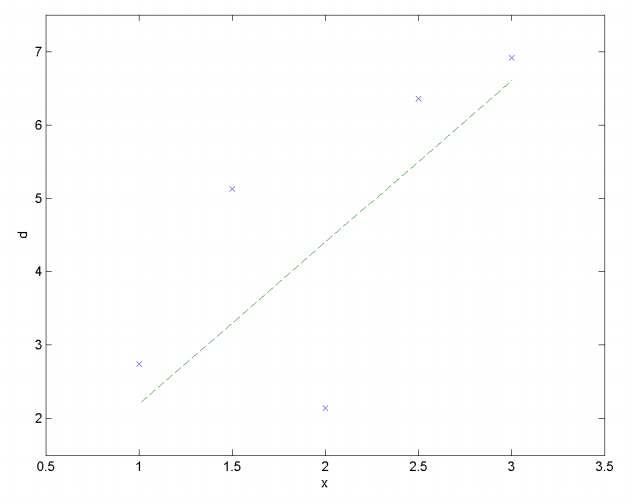
\includegraphics[width=0.80000\textwidth]{2018-03-10-10-00-53.png}\\

\end{frame}

\begin{frame}{Stochastic gradient descent error functions}

\centering 

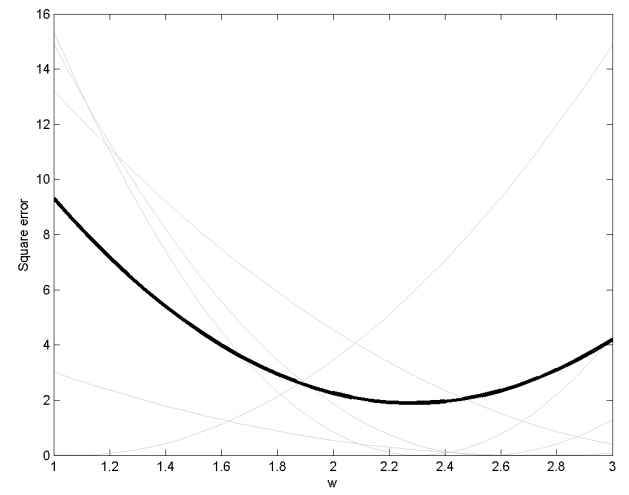
\includegraphics[width=0.80000\textwidth]{2018-03-10-10-01-05.png}\\

\end{frame}

\begin{frame}{Stochastic gradient descent gradients}

\centering 

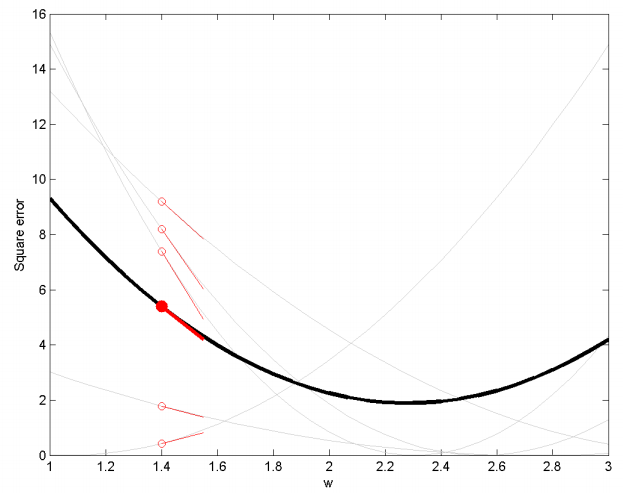
\includegraphics[width=0.80000\textwidth]{2018-03-10-10-01-13.png}\\

\end{frame}

\begin{frame}{Stochastic gradient descent animation}

\centering 

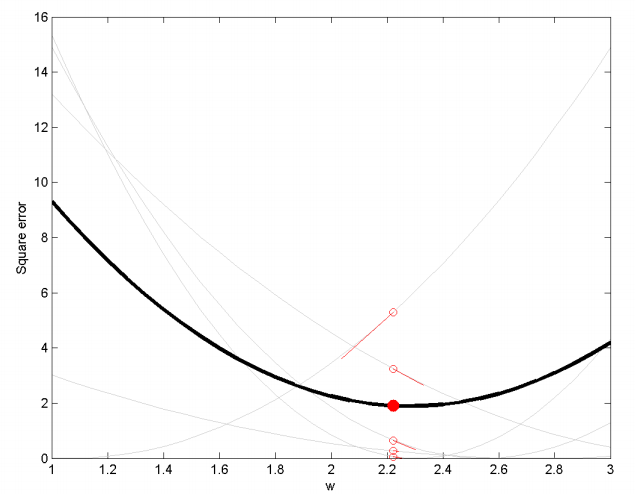
\includegraphics[width=0.80000\textwidth]{2018-03-10-10-01-21.png}\\

\end{frame}

\begin{frame}{Gradient descent animation}

\centering 

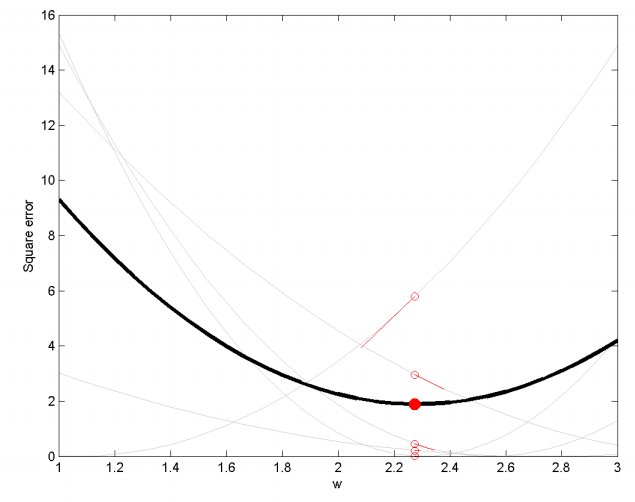
\includegraphics[width=0.80000\textwidth]{2018-03-10-10-01-33.png}\\

\end{frame}

\begin{frame}{Multi-variable LMS}

\begin{itemize}
\tightlist
\item
  The analysis for the one-variable case extends to the multi- variable
  case
\end{itemize}

\[ E ( n ) = 1/2 [d ( n ) - \vw^ T ( n )\vx( n )]^2 \]

\[  \nabla  E( w ) = \left(  \frac{\partial E}{\partial w_0}  ,  \frac{\partial E}{\partial w_1}  ,...,   \frac{\partial E}{\partial w_m} \right)^T \]

where \(w_0= b\) (bias) and \(x_0 = 1\), as done for perceptron learning

\end{frame}

\begin{frame}{Multi-variable LMS (cont.)}

\begin{itemize}
\tightlist
\item
  The LMS algorithm
\end{itemize}

\begin{eqnarray*}
    \vw ( n + 1)& =& \vw ( n )-\eta \nabla  \mE( n ) \\ 
    &= &\vw ( n ) + \eta e( n )\vx( n )\\
    &= &\vw ( n ) + \eta [d ( n ) - y ( n )]\vx( n ) 
\end{eqnarray*}

\end{frame}

\begin{frame}{LMS algorithm remarks}

\begin{itemize}
\tightlist
\item
  The LMS rule is exactly the same equation as the perceptron learning
  rule
\item
  Perceptron learning is for nonlinear (M-P) neurons, whereas LMS
  learning is for linear neurons.

  \begin{itemize}
  \tightlist
  \item
    \ie , perceptron learning is for classification and LMS is for
    function approximation
  \end{itemize}
\item
  LMS should be less sensitive to noise in the input data than
  perceptrons

  \begin{itemize}
  \tightlist
  \item
    On the other hand, LMS learning converges slowly
  \end{itemize}
\item
  Newtons method changes weights in the direction of the minimum
  \(E(w)\) and leads to fast convergence.

  \begin{itemize}
  \tightlist
  \item
    But it is not online and is computationally expensive
  \end{itemize}
\end{itemize}

\end{frame}

\begin{frame}{Stability of adaptation}

\begincols{}

\column{0.6\textwidth}

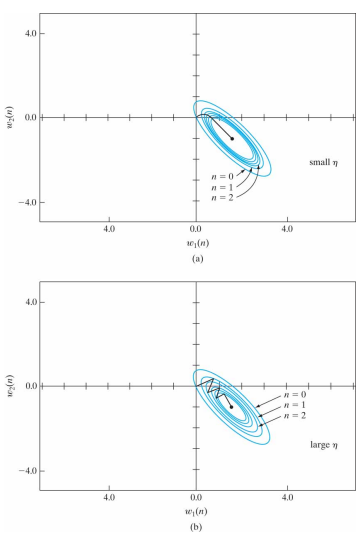
\includegraphics[width=0.80000\textwidth]{2018-03-10-10-13-18.png}\\

\column{0.4 \textwidth}

\begin{itemize}
\tightlist
\item
  When \(\eta\) is too small, learning converges slowly
\item
  When \(\eta\) is too large, learning does not converge
\end{itemize}

\stopcols

\end{frame}

\begin{frame}{Learning rate annealing}

\begin{itemize}
\item
  Basic idea: start with a large rate but gradually decrease it
\item
  Stochastic approximation \[\eta(n) = c/n\]

  \(c\) is a positive parameter
\end{itemize}

\end{frame}

\begin{frame}{Learning rate annealing (cont.)}

\begin{itemize}
\item
  Search-then-converge \[\eta(n) = \frac{\eta_0}{1+(n/\tau)}\]
  \(\eta_0\) and \(\tau\) are positive parameters

  \begin{itemize}
  \tightlist
  \item
    When \(n\) is small compared to \(\tau\) , learning rate is
    approximately constant
  \item
    When \(n\) is large compared to \(\tau\) , learning rule schedule
    roughly follows stochastic approximation
  \end{itemize}
\end{itemize}

\end{frame}

\begin{frame}{Rate annealing illustration}

\centering  

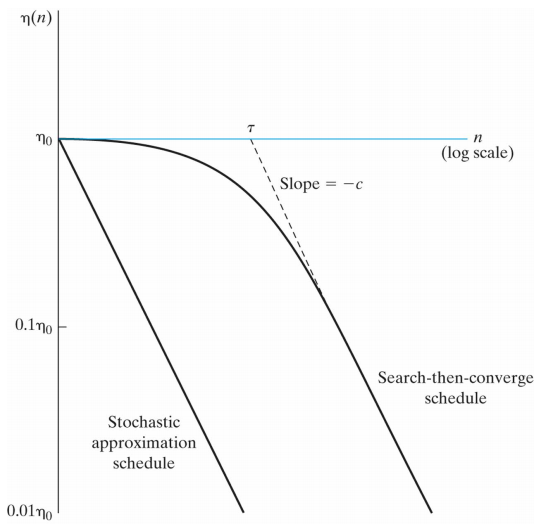
\includegraphics[width=0.70000\textwidth]{2018-03-10-10-18-17.png}\\

\end{frame}

\begin{frame}{Nonlinear neurons}

\begin{itemize}
\tightlist
\item
  To extend the LMS algorithm to nonlinear neurons, consider
  differentiable activation function at iteration n

  \begin{eqnarray*}
         E (n) &=& 1/2 \left[d (n)-  y (n)\right]^2 \\  
              &=& 1/2 \left[ d (n)  - \varphi \left( \sum_{j}  w_j x_j (n) \right) \right] ^2  
  \end{eqnarray*}
\end{itemize}

\end{frame}

\begin{frame}{Nonlinear neurons (cont.)}

\begin{itemize}
\tightlist
\item
  By chain rule of differentiation

  \begin{eqnarray*}
  \frac{\partial E}{\partial w_j} &=&
   \frac{\partial E}{\partial y}\frac{\partial y}{\partial v}\frac{\partial v}{\partial w_j} \\ 
  &=& - [d (n) - y (n)]\varphi' \left(v(n) \right)x_ j (n) \\ 
  &=& - e(n) \varphi' (v(n) ) x_ j (n)
  \end{eqnarray*}
\end{itemize}

\end{frame}

\begin{frame}{Nonlinear neurons (cont.)}

\begin{itemize}
\tightlist
\item
  Gradient descent gives

  \begin{eqnarray*}
     w _j (n + 1) &=& w_ j (n) +\eta e(n)\varphi' (v(n)) x _j (n) \\ 
                       &=& w_ j (n) +\eta \delta (n) x_ j (n) 
     \end{eqnarray*}

  \begin{itemize}
  \tightlist
  \item
    The above is called the delta (\(\delta\)) rule
  \end{itemize}
\item
  If we choose a logistic sigmoid for
  \[                    \varphi (v) = \frac{1}{  1+ exp( - av )} \] then
\end{itemize}

\[                   \varphi '      ( v ) = a \varphi ( v )[1-\varphi   ( v )]   \]

\end{frame}

\begin{frame}{Role of activation function}

\centering 

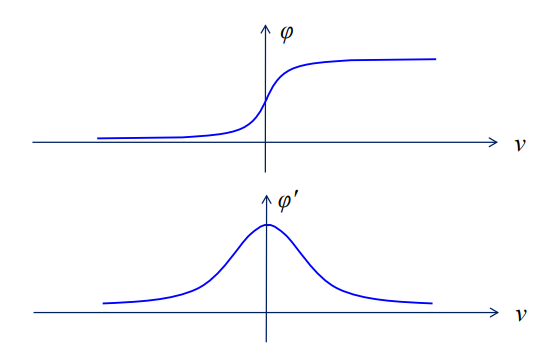
\includegraphics[width=1.00000\textwidth]{2018-03-10-10-41-52.png} ~

The role of \(\varphi'\): weight update is most sensitive when \(v\) is
near zero

\end{frame}

\begin{frame}
	\centering 
	\chuhao Thank you! %\fontspec{LHANDW.TTF}
\end{frame}


\end{document}
